\chapter{Overview on Graphene}
\label{grapheneTheory}
A snippet of graphene's electronic, geometrical and mechanical properties is available in the following sections.
\section{Theoretical snippets on graphene}
A single layer of graphene consists of a monolayer of carbon atoms arranged in a 2D honeycomb-like structure. Within each layer, every carbon atom bonds to three neighbouring carbon atoms building a quasi 2D plan~\cite{Neto2009}, with sp$^\textrm{2}$ hybridisation between carbon atoms resulting in the single layer of graphene being intact~\cite{Neto2009}. Each carbon atom within the graphene sheet has a dangling bond as it is only connected to three nearby carbon atoms leaving a free valence electron forming a cloud of electrons covering the single graphene sheet, organised in half filled $\pi$ orbitals~\cite{Neto2009}. Such carbon atom's $\pi$ orbital interacts with its neighbours' counterparts forming conduction and valence bands~\cite{Bolotin2008, Morozov2008, Basu2012}. Thus, graphene's band structure is due to those $\pi$ orbital electrons with the conduction and valence bands intersecting at a point in the Brillouin zone named Dirac point. Fig. \ref{fig:G_BSTRUCT_structure} shows the Dirac point with zero bandgap, confirming the semimetal nature of graphene~\cite{Wallace1947} characterised by the Dirac electrons. As a result, these $\pi$ orbital electrons cause graphene to be sensitive to the surroundings, paving the road towards graphene-based sensors~\cite{He2012, Mzali2016} as detailed in section \ref{graphene:sensor} with further explanation in Chapter \ref{grapheneSensors}.

%
\begin{figure}
    \centering
    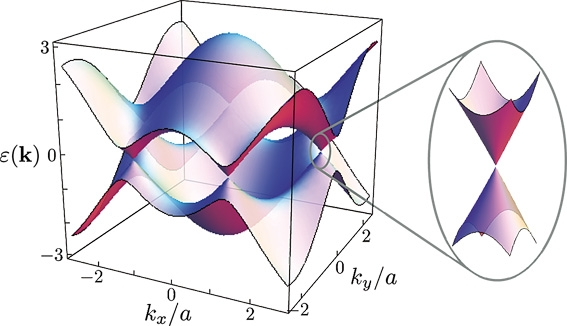
\includegraphics[width=\textwidth]{Figs/GrapheneBSTRUCT.png} %[scale=0.5,keepaspectratio]
    \caption{Graphene's band structure, from~\cite{dispersion}.}
    \label{fig:G_BSTRUCT_structure}
\end{figure}
%
Graphene monolayer sheet is considered one of the thinnest material ever known~\cite{Geim2007, Bunch2008}. Meanwhile, stacking graphene layers can take different stacking orders revealing different electronic properties. Two distinguished stacking orders can be either AA or AB stacking. AA stacking is semiconducting with a direct bandgap while AB stacking is a semi-metal with zero bandgap~\cite{Yakovkin2016}. In AA stacking order, the second layer's carbon atoms match precisely the top of the carbon atoms within the bottom layer. Within AB stacking, the carbon atoms within the top layer are on top of the centre of the honeycomb hexagon in the bottom layer. Figure (\ref{fig:G_BSTRUCT_structure_Stacking}) reveals the related band structure showing the band opening at the AA stacking order. Stability wise: AB stacking, which is the natural stacking order in graphite, is the more energetically favourable for graphene stacking orders~\cite{Yakovkin2016, Emroz2016, Cusati2017}. However, a forced opening of a bandgap in graphene's band structure can open many applications for graphene-based devices. Bandgap opening is possible through different techniques such as introducing strain in the graphene sheet~\cite{Zhen2008, Pereira2009, Cocco2010}, producing nanoribbons~\cite{Son2006, Han2007}, arrangement in different stacking orders~\cite{Ohta2006, Castro2007, Zhang2009}.
%
\begin{figure}
    \centering
    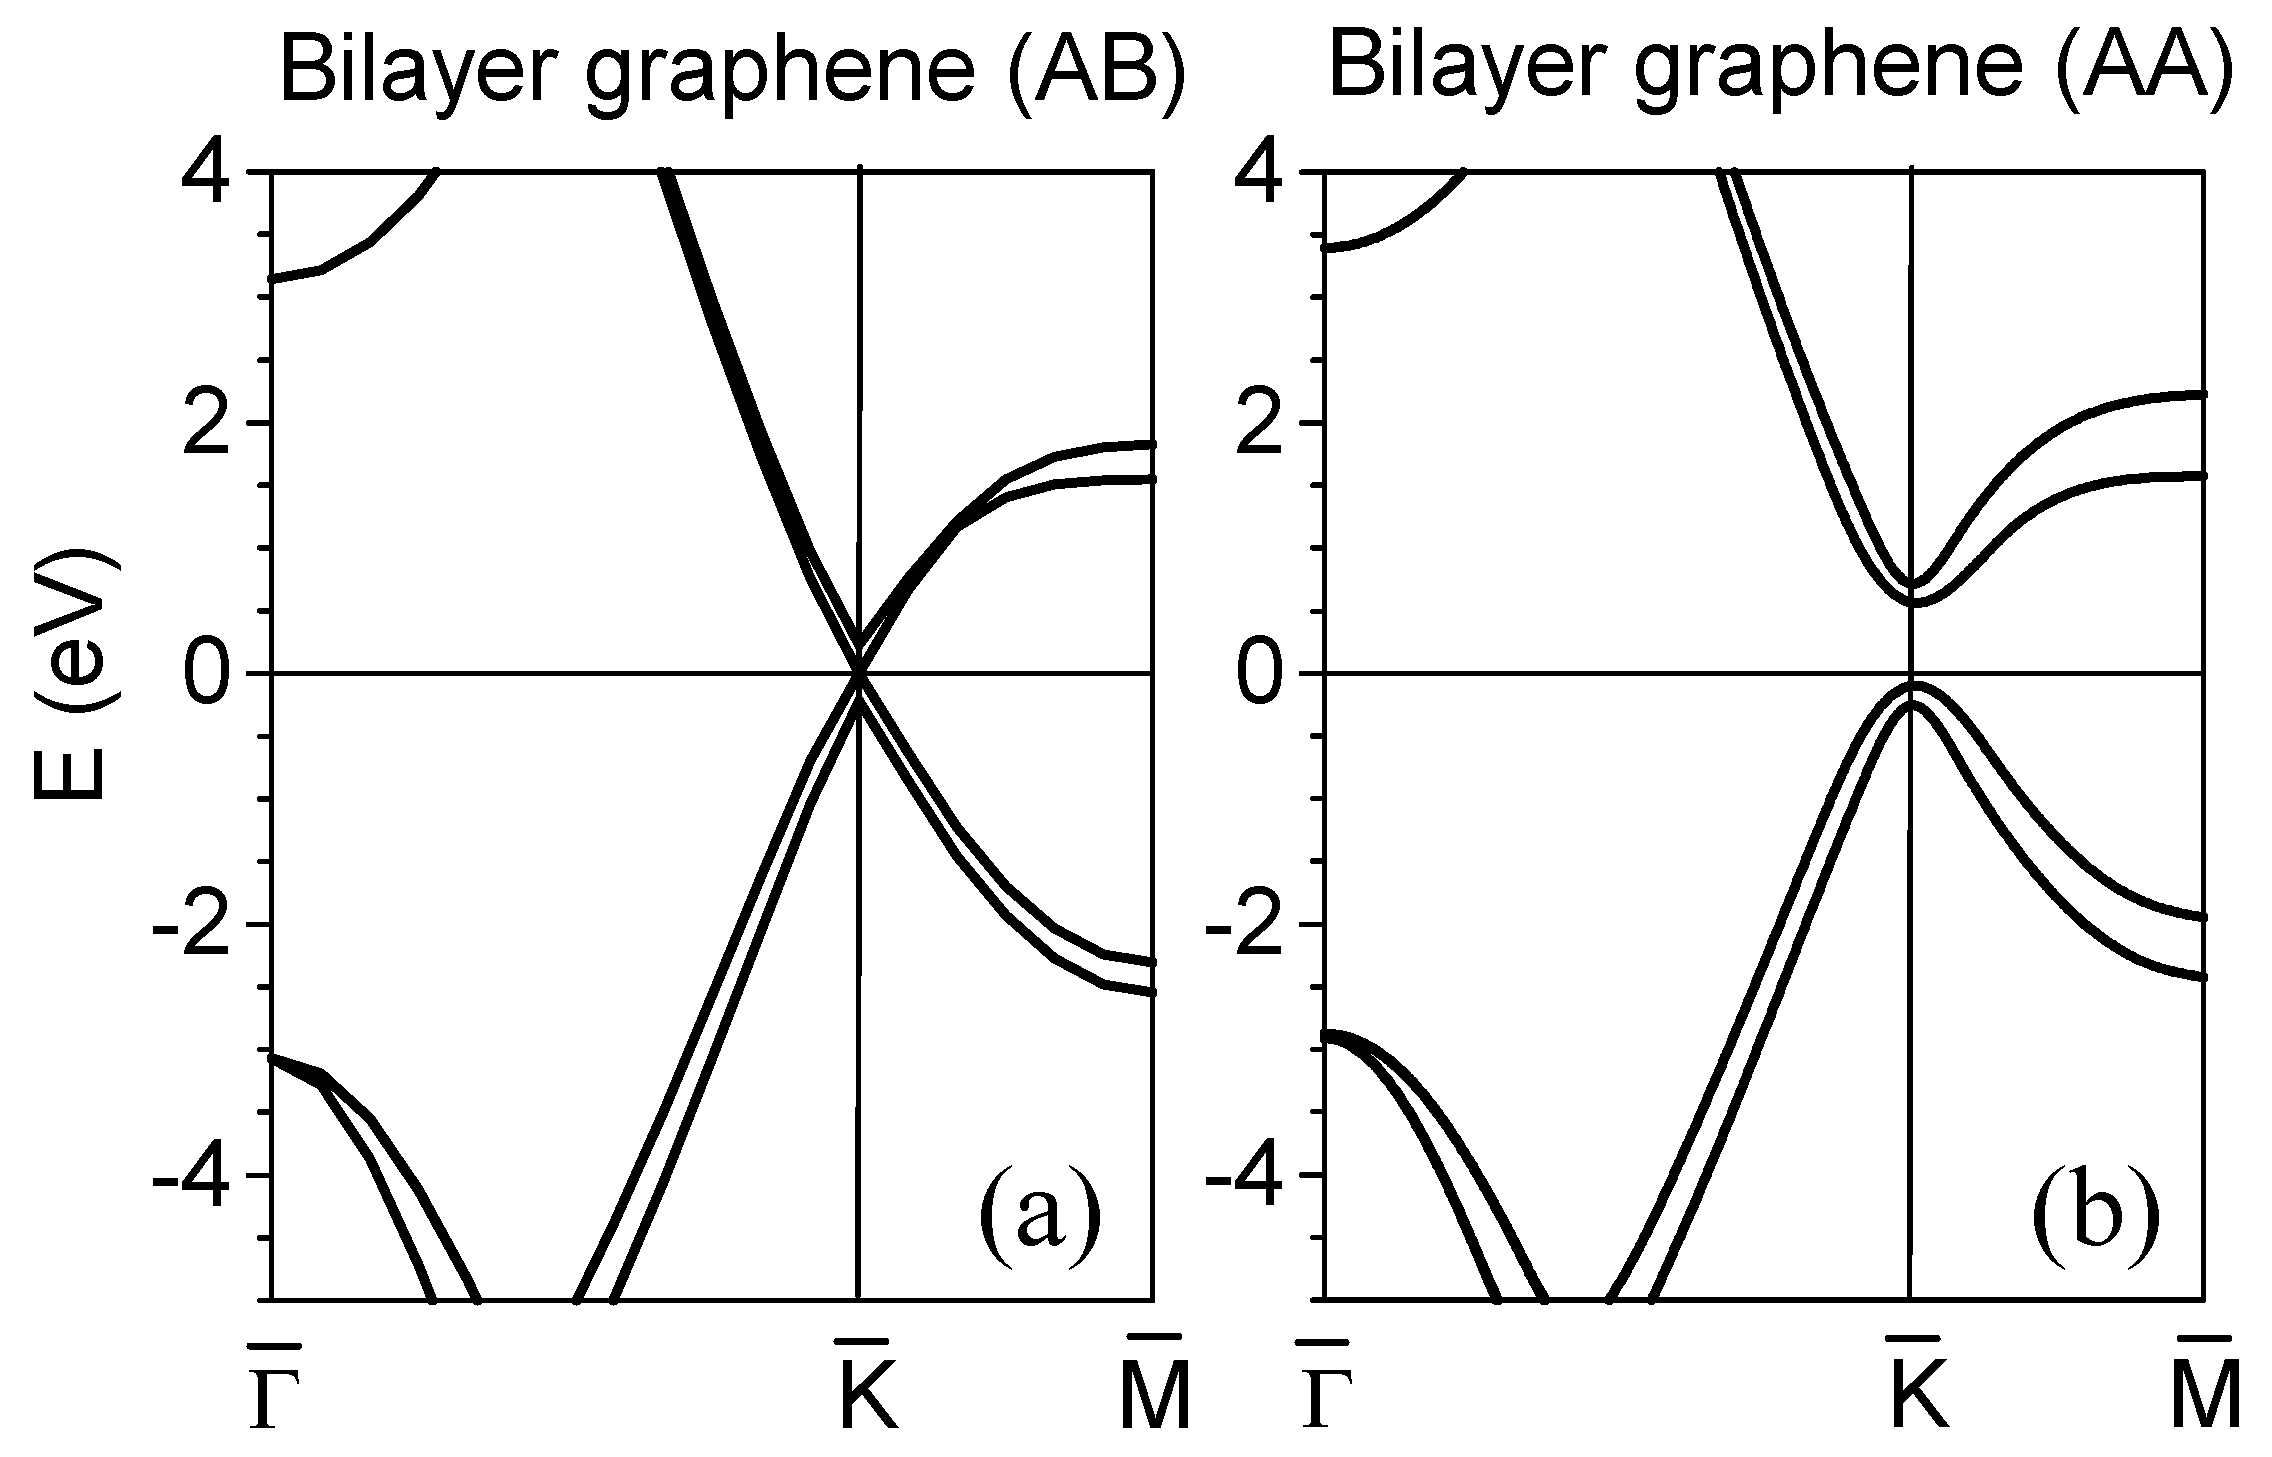
\includegraphics[width=\textwidth]{Figs/AA_AB_bandStructure.png}
    \caption{Band structure of AA and AB stacking orders in graphene bilayers. From~\cite{Yakovkin2016}}
    \label{fig:G_BSTRUCT_structure_Stacking}
\end{figure}

%
\subsection{Electronic properties}
\label{graphene:electronic}
Graphene shows ballistic transport due to the Dirac fermions that are massless quasiparticles~\cite{Geim2007}. Those massless quasiparticles are responsible for the resultant graphene's band structure (depicted in Fig. \ref{fig:G_BSTRUCT_structure}). They are a result of the graphene's electrons interacting with the hexagonal lattice periodic potential~\cite{Geim2007}. The Dirac equation~\cite{Gusynin2005, Novoselov2005, Zhang2005, Geim2007} does accurately model those particles. They are the graphene's charge carriers, and their relativistic properties are investigated experimentally via quantum Hall effect measurements~\cite{Novoselov2004, Novoselov2005}. Experimental studies~\cite{Novoselov2004, Hwang2007, Bolotin2008, Morozov2008, Vincent2010, Rahimi2014, Banszeruse2015} shows high mobility of 200,000 $\textrm{cm}^2 \textrm{V}^{-1}\textrm{s}^{-1}$. Moreover, graphene has been proven to have a low electronic noise, which in turn makes it an ideal material for detecting adsorbant gas molecules on its surface~\cite{Schedin2007}. Further details are discussed in the following chapter regarding the detection and sensing properties of graphene.
%
\subsection{Mechanical properties}
Graphene's mechanical properties are outstanding. Graphene has a Young modulus of 1 TPa~\cite{Lee2008, Lee2013} qualifying it to be part of nanoelectromechanical systems (NEMS) and electromechanical transducers~\cite{Smith2013, Smith2016a}. Applying strain of 20 \% is possible on graphene while maintaining the elastic region~\cite{Tomori2011}.  In turn, this opens the possibility for applications of graphene-based devices in the flexible electronics world~\cite{Fiori2014nature}. Moreover, applying strain can open a bandgap~\cite{Cocco2010}, with a shift in the Dirac point~\cite{Montambaux2009, Pereira2009, Li2014} and hence a bandgap in the resultant band structure of the graphene sheet. Furthermore, graphene well-reside on top of silica substrates~\cite{Koenig2011, Rudenko2011, Zhao2017} with strong adhesion forces dominated by van der Waals dispersive interactions. Finally, Graphene can build impermeable membranes, where it reported impermeability to standard gases~\cite{Bunch2008}. That is advantageous when designing graphene-based sensors.
%
\section{Graphene's applications}
Graphene faces some complications in the fabrication and design processes~\cite{Smith2016a, Fiori2014nature}, yet it is quite paying back concerning its wide applications integrity due to its extraordinary properties discussed earlier. This pool of applications for such a 2D material and other challenging 2D materials include, but not limited to, transistors~\cite{Lemme2012, Lemme2012a}, sensors~\cite{Smith2015, Smith2016a, Smith2017, Xuge2017, Feng2014, Wang2015, Yue2013, Zhao2014, Llobet2013}, transistor passivation~\cite{Smith2016}, energy harvesting~\cite{GRANDE2012}, faster charging batteries~\cite{Son2017}, potentiometer~\cite{Levesque2011}, supercapacitors and energy storage~\cite{Yoo2011, Brownson2012, Liu2010}, photodetectors~\cite{Mueller2010, Naiini2014, Lemme2011}, photodiodes~\cite{Riazimehr2017}, analog electronics~\cite{Fiori2014}, solar cells~\cite{Wang2008, Miao2012}, RF devices~\cite{Fiori2014nature}. Graphene's high optical transparency and high electronic conductivity open the door for touch screens~\cite{Ferrari2015} as a direct application of optoelectronic devices. Graphene applications can be extend towards NEMS systems~\cite{Chen2013}, such as graphene-based mechanical resonators~\cite{Bunch2007, Castellanos2015, Chen2013}, cantilevers~\cite{Conley2011}, pressure sensors~\cite{Smith2012, Smith2013b, Smith2014, Wagner2016}, magnetic field sensors~\cite{Dauber2015}, accelerometers~\cite{memsPatent}. All these applications fall into \textit{more than Moore} paradigm.
\subsection{Transistors}
Graphene can build the channel material in transistors for a promising post-silicon field effect transistor (FET) devices~\cite{Lemme2007, Smith2016a}. In such devices, the current flow in the central channel region from the source to the drain electrodes. This current is controlled by applying an external voltage to the gate electrode, which is shielded against the channel region by a dielectric. Applying means of external electric field can alter Graphene's resistance opening the possibilities for high-speed transistors~\cite{Schwierz2010}. Graphene can also be part of the base component of the transistor in graphene-based bipolar junction transistor (BJT)~\cite{Vaziri2013}. Graphene transistors can act as amplifiers as in~\cite{Han2011}. Graphene can be a promising building block for high-frequency devices for communication purposes~\cite{Smith2016a, Liao2012}. On a circuit design level, circuits designs can model and simulate graphene-based circuit components~\cite{Han2011, Wu2012, Thiele2010, Fregonese2013, Rodriguez2014}.
\subsection{Sensors}
\label{graphene:sensor}
Graphene has demonstrated potential in the sensor field due to its extraordinary properties, discussed in section \ref{graphene:electronic}. One of the main sensor applications here is the gas sensor in the form of solid-state devices featuring graphene~\cite{Moseley1997, Handbook_gas_sensing, Capone2003, Smith2016a, Elgammal2016Lic}. Such devices demonstrate competitive edge with sensing applications for more NEMS based applications. Chapter \ref{grapheneSensors} details the sensing action of graphene.
\section{Summary}
In summary, graphene has shown the potential to be a key player in advancing material science due to its remarkable properties being either electric or mechanical. Such properties allow graphene to be implemented in a wide range of device applications either being electronic or mechanical or consolidating both. Besides, being CMOS compatible allows it to be embedded in the current technologies seamlessly.
\endinput